\chapter{Results}\label{chap:results}
In this chapter, the results of implementing \acrlong{ML} algorithms, discussed in chapter \ref{chap:method} are given, followed by a comparison of their performance and computational complexity.

The upcoming results were achieved under the following conditions:

\begin{itemize}
    \item The test set comprises 25\% of the initial dataset.
    \item \acrlong{SMOTE} is used to balance the skewed distribution.
    \item A 5-fold cross-validation with three repetitions is used to assess our method. Hence, the average of 15 test results is used to evaluate the effect of various methods' classification.
    \item Six criteria are used to evaluate each model: \acrlong{AUC}, Accuracy, Precision, Recall, F1-score, and Cohen's Kappa.
\end{itemize}

{\hskip 1em} Additionally, there are four more statistics obtained from each experiment and these form the Confusion Matrix. These parameters are used to calculate the metrics mentioned above (excluding Cohen's Kappa), as presented in \crefrange{eq:accu}{eq:f1sc}:

\begin{table}[H]
% \centering
\setlength\tabcolsep{5pt}
\begin{tabular}{@{}ll@{}}
\textbf{\textit{True Positive (TP):}}  & the patient is alive at the discharge time, and the prediction is \textsc{Alive}.              \\ 
\textbf{\textit{True Negative (TN):}}  & the patient died in hospital, and the prediction is \textsc{Expired}.                    \\ 
\textbf{\textit{False Positive (FP):}} & the patient is alive at the discharge time, but the prediction is \textsc{Expired}. \\ 
\textbf{\textit{False Negative (FN):}} & the patient died in hospital while the prediction is \textsc{Alive}.                      \\
\end{tabular}
\label{tab:confusionmatparam}
\vspace{-3mm}
\end{table}

{\hskip 1em} Classification accuracy, \cref{eq:accu}, is the ability of classifiers to make accurate predictions. To calculate \acrfull{ROC}, sensitivity, \cref{eq:sens}, and specificity, \cref{eq:spec}, must be obtained to draw \acrfull{AUC} for each model. In the \acrshort{ROC} curve, the horizontal axis is \textit{FPR}, and the vertical axis is \textit{TPR}. Hence, the closer the distance of the point on the \acrshort{ROC} curve to (0, 1), the
higher the classifier's accuracy \cite{ma_gradient_2019}. When instances are balanced between each class, using the \acrshort{ROC} curve is the right choice. On the contrary, the \textsc{Precision-Recall} curve is appropriate for imbalanced datasets.

{\hskip 1em} \textit{F1-score}, \cref{eq:f1sc}, computes the harmonic mean of the \textit{Precision} and \textit{Recall}. For a specific probability threshold (e.g., 0.5), \textit{F1-score} summarizes model skill, whereas the \acrlong{AUC} summarizes the skill of a model across thresholds \cite{brownlee_master_2016}.

\begin{align}
    Accuracy \ & = \ \frac{TP + TN}{TP + TN + FP + FN} \label{eq:accu} \\[10pt] 
    Sensitivity \ or \ TPR \ & = \ \frac{TP}{TP + FN}  \label{eq:sens} \\[10pt]
    Specificity \ or \ FPR \ & = \ \frac{FP}{FP + TN}  \label{eq:spec} \\[10pt]
    Precision \ & = \ \frac{TP}{TP + FP}               \label{eq:prec} \\[10pt]
    Recall \ & = \ \frac{TP}{TP + FN}                  \label{eq:recl} \\[10pt]
    F1-score \ & = \ \frac{2 \times Precision \times Recall}{Precision + Recall} \label{eq:f1sc}
\end{align} 

\smallskip
{\hskip 1em} \cref{fig:cartconfusionmat,fig:xgbconfusionmat,fig:svmconfusionmat,fig:lrconfusionmat,fig:nbconfusionmat,fig:ldaconfusionmat,fig:knnconfusionmat} show the Confusion Matrices obtained from the four pre-discussed parameters, \textit{TP}, \textit{TN}, \textit{FP}, and \textit{FN}, for all the implemented algorithms. The more the predictions fall on the matrix's diagonal line, the better the performance of our model is. \

{\hskip 1em} \crefrange{tab:cartreport}{tab:knnreport} provide detailed information about the usage of \cref{eq:accu,eq:prec,eq:recl,eq:f1sc} in our chosen models for each class. \

{\hskip 1em} The \acrshort{ROC} curve of each algorithm is shown in \cref{fig:cartroc,fig:xgbroc,fig:svmroc,fig:lrroc,fig:nbroc,fig:ldaroc,fig:knnroc}, while their respective \textsc{Precision-Recall} curve is depicted in \cref{fig:cartprerec,fig:xgbprerec,fig:svmprerec,fig:lrprerec,fig:nbprerec,fig:ldaprerec,fig:knnprerec}. As it can also be seen in \crefrange{eq:prec}{eq:recl}, \textsc{Precision-Recall} curves do not consider \textit{TN}.\

{\hskip 1em} All the corresponding developed codes that brought about this chapter's results can be found in the author's profile on GitHub repository\footnote{\href{https://github.com/mani0098/GlucoseLactateMortality}{https://github.com/mani0098/GlucoseLactateMortality}}.

\clearpage
\section{Implemented CART Results}

\begin{table}[h]
\fontfamily{pcr}\selectfont
\centering
\setlength\tabcolsep{10pt}
\caption{\label{tab:cartreport}The classification report of the \acrshort{CART} algorithm}
\resizebox{0.7\textwidth}{!}{%
\begin{tabular}{@{}rrrrr@{}}
\thead{} & \thead{precision} & \thead{recall} & \thead{f1-score} & \thead{support} \\ [12pt]
Alive         & 0.83  & 0.87  & 0.85  & 12058       \\ 
Expired       & 0.86  & 0.82  & 0.84  & 11990       \\ 
                                                    \\
accuracy      &       &       & 0.84  & 24048       \\ 
micro avg     & 0.84  & 0.84  & 0.84  & 24048       \\
weighted avg  & 0.84  & 0.84  & 0.84  & 24048       \\
\end{tabular}}
\end{table}

\begin{figure}[H]
\centering
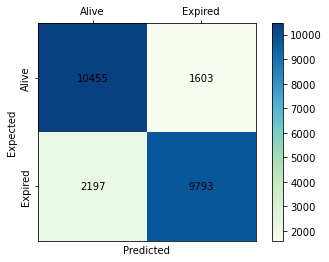
\includegraphics[width=8cm]{fig/chapter5/CART/Confusion Matrix_new.png}
\caption{Confusion matrix for the \acrshort{CART} algorithm}
\label{fig:cartconfusionmat}
\end{figure}

\begin{figure}[H]
\begin{tabular}{@{}cc@{}}
\begin{subfigure}{0.5\textwidth}
  \centering
  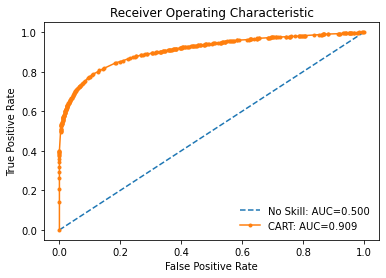
\includegraphics[width=7.5cm]{fig/chapter5/CART/ROC_new.png}
  \caption{\footnotesize{The \acrshort{ROC} curve}}
  \label{fig:cartroc}
\end{subfigure} 
\begin{subfigure}{0.5\textwidth}
  \centering
  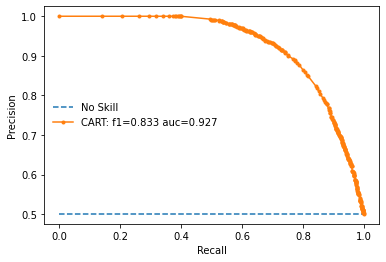
\includegraphics[width=7.5cm]{fig/chapter5/CART/Precision-Recall_new.png}
  \caption{\footnotesize{The Precision-Recall curve}}
  \label{fig:cartprerec}
\end{subfigure} \\
\end{tabular}
\caption{Curves of \acrshort{ROC} and Precision-Recall using the \acrshort{CART} algorithm}
\label{fig:cartcurves}
\end{figure}

\section{Implemented XGBoost Results}

\begin{table}[h]
\fontfamily{pcr}\selectfont
\centering
\setlength\tabcolsep{10pt}
\caption{\label{tab:xgbreport}The classification report of the \acrshort{XGB} algorithm}
\resizebox{0.7\textwidth}{!}{%
\begin{tabular}{@{}rrrrr@{}}
\thead{} & \thead{precision} & \thead{recall} & \thead{f1-score} & \thead{support} \\ [12pt]
Alive         & 0.88  & 0.94  & 0.91  & 12069       \\ 
Expired       & 0.93  & 0.87  & 0.90  & 11979       \\ 
                                                    \\
accuracy      &       &       & 0.90  & 24048       \\ 
micro avg     & 0.90  & 0.90  & 0.90  & 24048       \\
weighted avg  & 0.90  & 0.90  & 0.90  & 24048       \\
\end{tabular}}
\end{table}

\begin{figure}[H]
\centering
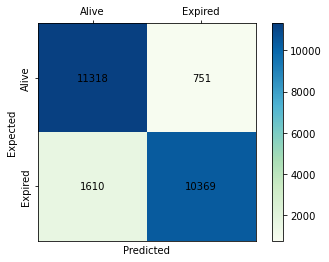
\includegraphics[width=8cm]{fig/chapter5/XGB/Confusion_Matrix_new.png}
\caption{Confusion matrix for the \acrshort{XGB} algorithm}
\label{fig:xgbconfusionmat}
\end{figure}

\begin{figure}[H]
\begin{tabular}{@{}cc@{}}
\begin{subfigure}{0.5\textwidth}
  \centering
  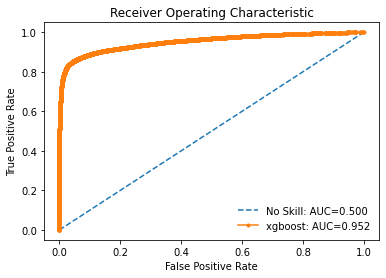
\includegraphics[width=7.5cm]{fig/chapter5/XGB/ROC_new.png}
  \caption{\footnotesize{The \acrshort{ROC} curve}}
  \label{fig:xgbroc}
\end{subfigure} 
\begin{subfigure}{0.5\textwidth}
  \centering
  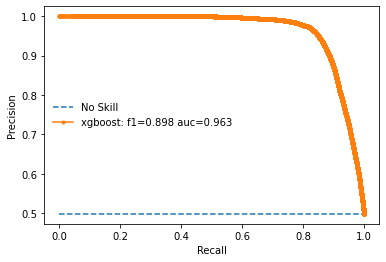
\includegraphics[width=7.5cm]{fig/chapter5/XGB/Precision-Recall_new.png}
  \caption{\footnotesize{The Precision-Recall curve}}
  \label{fig:xgbprerec}
\end{subfigure} \\
\end{tabular}
\caption{Curves of \acrshort{ROC} and Precision-Recall using the \acrshort{XGB} algorithm}
\label{fig:xgbcurves}
\end{figure}

\section{Implemented SVM Results}

\begin{table}[h]
\fontfamily{pcr}\selectfont
\centering
\setlength\tabcolsep{10pt}
\caption{\label{tab:svmreport}The classification report of the \acrshort{SVM} algorithm}
\resizebox{0.7\textwidth}{!}{%
\begin{tabular}{@{}rrrrr@{}}
\thead{} & \thead{precision} & \thead{recall} & \thead{f1-score} & \thead{support} \\ [12pt]
Alive         & 0.66  & 0.80  & 0.72  & 12130       \\ 
Expired       & 0.74  & 0.58  & 0.65  & 11918       \\ 
                                                    \\
accuracy      &       &       & 0.69  & 24048       \\ 
micro avg     & 0.70  & 0.69  & 0.69  & 24048       \\
weighted avg  & 0.70  & 0.69  & 0.69  & 24048       \\
\end{tabular}}
\end{table}

\begin{figure}[H]
\centering
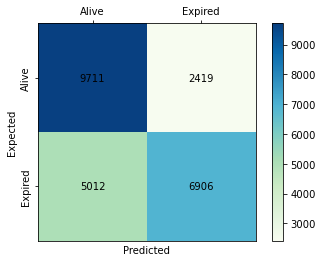
\includegraphics[width=8cm]{fig/chapter5/SVM/Confusion Matrix_new.png}
\caption{Confusion matrix for the \acrshort{SVM} algorithm}
\label{fig:svmconfusionmat}
\end{figure}

\begin{figure}[H]
\begin{tabular}{@{}cc@{}}
\begin{subfigure}{0.5\textwidth}
  \centering
  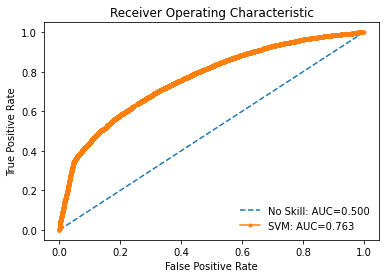
\includegraphics[width=7.5cm]{fig/chapter5/SVM/ROC_new.png}
  \caption{\footnotesize{The \acrshort{ROC} curve}}
  \label{fig:svmroc}
\end{subfigure} 
\begin{subfigure}{0.5\textwidth}
  \centering
  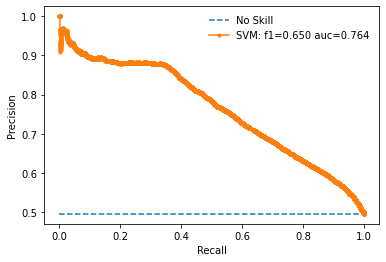
\includegraphics[width=7.5cm]{fig/chapter5/SVM/Precision-Recall_new.png}
  \caption{\footnotesize{The Precision-Recall curve}}
  \label{fig:svmprerec}
\end{subfigure} \\
\end{tabular}
\caption{Curves of \acrshort{ROC} and Precision-Recall using the \acrshort{SVM} algorithm}
\label{fig:svmcurves}
\end{figure}

\section{Implemented Logistic Regression Results}

\begin{table}[h]
\fontfamily{pcr}\selectfont
\centering
\setlength\tabcolsep{10pt}
\caption{\label{tab:lrreport}The classification report of the \acrlong{LR} algorithm}
\resizebox{0.7\textwidth}{!}{%
\begin{tabular}{@{}rrrrr@{}}
\thead{} & \thead{precision} & \thead{recall} & \thead{f1-score} & \thead{support} \\ [12pt]
Alive         & 0.66  & 0.75  & 0.70  & 12031       \\ 
Expired       & 0.71  & 0.61  & 0.65  & 12017       \\ 
                                                    \\
accuracy      &       &       & 0.68  & 24048       \\ 
micro avg     & 0.68  & 0.68  & 0.68  & 24048       \\
weighted avg  & 0.68  & 0.68  & 0.68  & 24048       \\
\end{tabular}}
\end{table}

\begin{figure}[H]
\centering
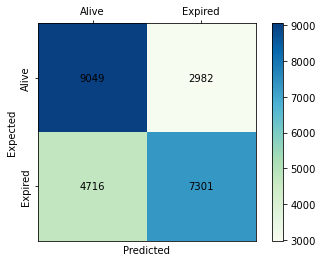
\includegraphics[width=8cm]{fig/chapter5/LR/Confusion Matrix_new.png}
\caption{Confusion matrix for the \acrshort{LR} algorithm}
\label{fig:lrconfusionmat}
\end{figure}

\begin{figure}[H]
\begin{tabular}{@{}cc@{}}
\begin{subfigure}{0.5\textwidth}
  \centering
  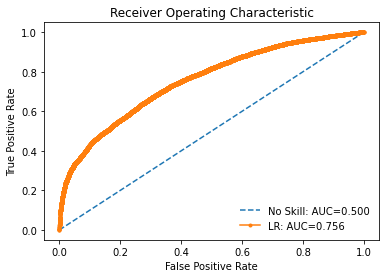
\includegraphics[width=7.5cm]{fig/chapter5/LR/ROC_new.png}
  \caption{\footnotesize{The \acrshort{ROC} curve}}
  \label{fig:lrroc}
\end{subfigure} 
\begin{subfigure}{0.5\textwidth}
  \centering
  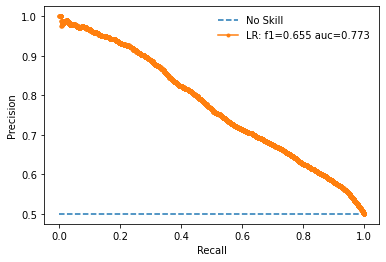
\includegraphics[width=7.5cm]{fig/chapter5/LR/Precision-Recall_new.png}
  \caption{\footnotesize{The Precision-Recall curve}}
  \label{fig:lrprerec}
\end{subfigure} \\
\end{tabular}
\caption{Curves of \acrshort{ROC} and Precision-Recall using the \acrlong{LR} algorithm}
\label{fig:lrcurves}
\end{figure}

\section{Implemented Na\"ive Bayes Results}

\begin{table}[h]
\fontfamily{pcr}\selectfont
\centering
\setlength\tabcolsep{10pt}
\caption{\label{tab:nbreport}The classification report of the \acrlong{NB} algorithm}
\resizebox{0.7\textwidth}{!}{%
\begin{tabular}{@{}rrrrr@{}}
\thead{} & \thead{precision} & \thead{recall} & \thead{f1-score} & \thead{support} \\ [12pt]
Alive         & 0.60  & 0.92  & 0.73  & 12028       \\ 
Expired       & 0.83  & 0.39  & 0.53  & 12020       \\ 
                                                    \\
accuracy      &       &       & 0.65  & 24048       \\ 
micro avg     & 0.72  & 0.65  & 0.63  & 24048       \\
weighted avg  & 0.72  & 0.65  & 0.63  & 24048       \\
\end{tabular}}
\end{table}

\begin{figure}[H]
\centering
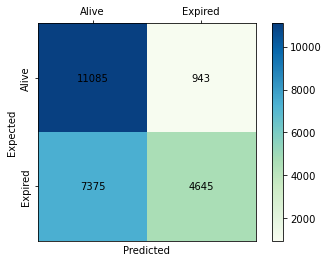
\includegraphics[width=8cm]{fig/chapter5/NB/Confusion Matrix_new.png}
\caption{Confusion matrix for the \acrlong{NB} algorithm}
\label{fig:nbconfusionmat}
\end{figure}

\begin{figure}[H]
\begin{tabular}{@{}cc@{}}
\begin{subfigure}{0.5\textwidth}
  \centering
  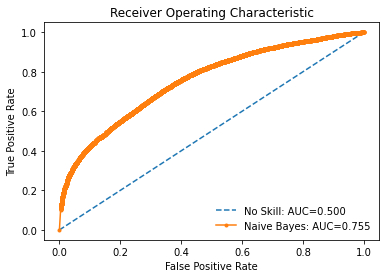
\includegraphics[width=7.5cm]{fig/chapter5/NB/ROC_new.png}
  \caption{\footnotesize{The \acrshort{ROC} curve}}
  \label{fig:nbroc}
\end{subfigure} 
\begin{subfigure}{0.5\textwidth}
  \centering
  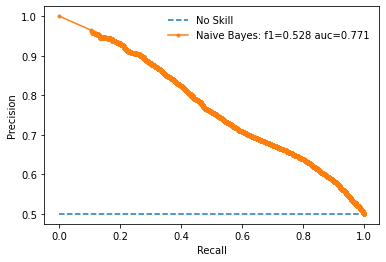
\includegraphics[width=7.5cm]{fig/chapter5/NB/Precision-Recall_new.png}
  \caption{\footnotesize{The Precision-Recall curve}}
  \label{fig:nbprerec}
\end{subfigure} \\
\end{tabular}
\caption{Curves of \acrshort{ROC} and Precision-Recall using the \acrlong{NB} algorithm}
\label{fig:nbcurves}
\end{figure}

\section{Implemented LDA Results}

\begin{table}[h]
\fontfamily{pcr}\selectfont
\centering
\setlength\tabcolsep{10pt}
\caption{\label{tab:ldareport}The classification report of the \acrshort{LDA} algorithm}
\resizebox{0.7\textwidth}{!}{%
\begin{tabular}{@{}rrrrr@{}}
\thead{} & \thead{precision} & \thead{recall} & \thead{f1-score} & \thead{support} \\ [12pt]
Alive         & 0.65  & 0.76  & 0.70  & 12093       \\ 
Expired       & 0.71  & 0.59  & 0.65  & 11955       \\ 
                                                    \\
accuracy      &       &       & 0.68  & 24048       \\ 
micro avg     & 0.68  & 0.68  & 0.67  & 24048       \\
weighted avg  & 0.68  & 0.68  & 0.67  & 24048       \\
\end{tabular}}
\end{table}

\begin{figure}[H]
\centering
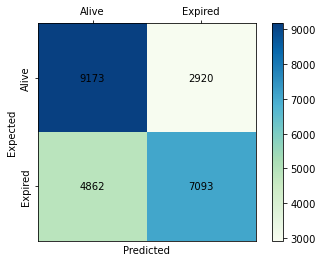
\includegraphics[width=8cm]{fig/chapter5/LDA/Confusion Matrix_new.png}
\caption{Confusion matrix for the \acrshort{LDA} algorithm}
\label{fig:ldaconfusionmat}
\end{figure}

\begin{figure}[H]
\begin{tabular}{@{}cc@{}}
\begin{subfigure}{0.5\textwidth}
  \centering
  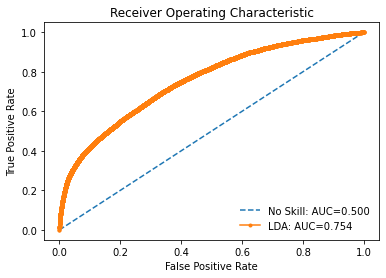
\includegraphics[width=7.5cm]{fig/chapter5/LDA/ROC_new.png}
  \caption{\footnotesize{The \acrshort{ROC} curve}}
  \label{fig:ldaroc}
\end{subfigure} 
\begin{subfigure}{0.5\textwidth}
  \centering
  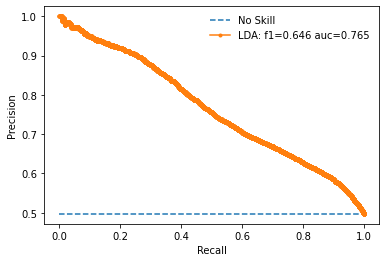
\includegraphics[width=7.5cm]{fig/chapter5/LDA/Precision-Recall_new.png}
  \caption{\footnotesize{The Precision-Recall curve}}
  \label{fig:ldaprerec}
\end{subfigure} \\
\end{tabular}
\caption{Curves of \acrshort{ROC} and Precision-Recall using the \acrshort{LDA} algorithm}
\label{fig:ldacurves}
\end{figure}

\section{Implemented KNN Results}

\begin{table}[h]
\fontfamily{pcr}\selectfont
\centering
\setlength\tabcolsep{10pt}
\caption{\label{tab:knnreport}The classification report of the \acrlong{KNN} algorithm}
\resizebox{0.7\textwidth}{!}{%
\begin{tabular}{@{}rrrrr@{}}
\thead{} & \thead{precision} & \thead{recall} & \thead{f1-score} & \thead{support} \\ [12pt]
Alive         & 0.92  & 0.69  & 0.79  & 12147       \\ 
Expired       & 0.75  & 0.94  & 0.83  & 11901       \\ 
                                                    \\
accuracy      &       &       & 0.82  & 24048       \\ 
micro avg     & 0.84  & 0.82  & 0.81  & 24048       \\
weighted avg  & 0.84  & 0.82  & 0.81  & 24048       \\
\end{tabular}}
\end{table}

\begin{figure}[H]
\centering
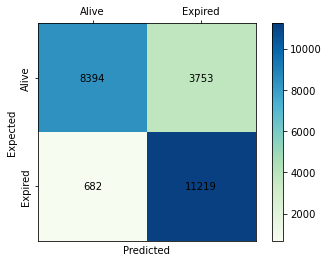
\includegraphics[width=8cm]{fig/chapter5/KNN/Confusion Matrix_new.png}
\caption{Confusion matrix for the \acrshort{KNN} algorithm}
\label{fig:knnconfusionmat}
\end{figure}

\begin{figure}[H]
\begin{tabular}{@{}cc@{}}
\begin{subfigure}{0.5\textwidth}
  \centering
  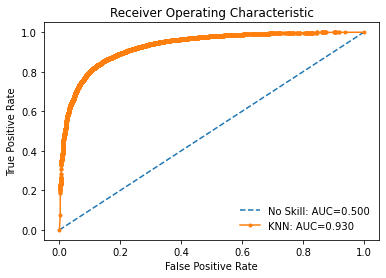
\includegraphics[width=7.5cm]{fig/chapter5/KNN/ROC_new.png}
  \caption{\footnotesize{The \acrshort{ROC} curve}}
  \label{fig:knnroc}
\end{subfigure} 
\begin{subfigure}{0.5\textwidth}
  \centering
  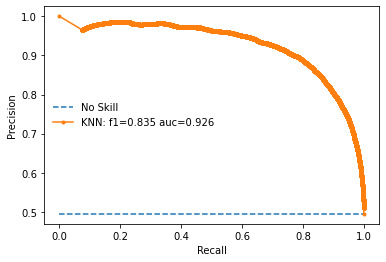
\includegraphics[width=7.5cm]{fig/chapter5/KNN/Precision-Recall_new.png}
  \caption{\footnotesize{The Precision-Recall curve}}
  \label{fig:knnprerec}
\end{subfigure} \\
\end{tabular}
\caption{Curves of \acrshort{ROC} and Precision-Recall using the \acrshort{KNN} algorithm}
\label{fig:knncurves}
\end{figure}

\section{Discussion}

\subsection{Comparison}
Given all the results for the seven different \acrshort{ML} algorithms, \crefrange{tab:cartreport}{tab:knnreport} and \crefrange{fig:cartconfusionmat}{fig:knncurves}, it is easy to deduce that \acrshort{XGB} outperforms the other algorithms. Even though our primary metric for model evaluation was \acrlong{AUC}, \acrshort{XGB} retains its supremacy in accuracy and \acrshort{AUC} in \textsc{Precision-Recall} curves. This outcome is achieved mainly because of the inherent power of the Decision-Tree-based algorithms in solving binary class problems, and also due to not having any missing data in our dataset along with applying \acrshort{SMOTE} to balance the skewed cohort. Figure \ref{fig:comparison} shows how much applying a resampling algorithm matters. When no \acrshort{SMOTE} is applied, \crefrange{fig:rskfoldnosmote}{fig:skfoldnosmote}, \acrshort{SVM} results in slightly better than the rest of the algorithms concerning \acrshort{AUC}. In contrast, when \acrshort{SMOTE} is employed, \crefrange{fig:rskfoldsmote}{fig:skfoldsmote}, \acrshort{XGB}, \acrshort{KNN}, and \acrshort{CART} become the premier models. It can also be derived from figure \ref{fig:comparison} that methods like \acrshort{LR}, \acrshort{LDA}, \acrshort{NB}, and \acrshort{SVM} are indifferent to \acrshort{SMOTE}, while \acrshort{KNN}, \acrshort{CART}, and \acrshort{XGB} are significantly affected by it.

\begin{figure}[H]
\begin{tabular}{@{}cc@{}}
\begin{subfigure}{0.5\textwidth}
  \centering
  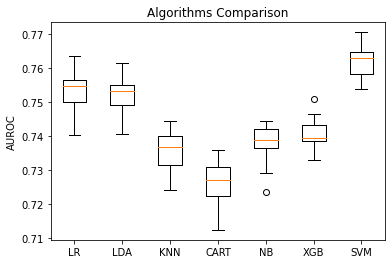
\includegraphics[width=7.5cm]{fig/chapter5/Algorithm Comparison (no SMOTE, RSKFold).png}
  \caption{\footnotesize{Repeated 5-fold cross-validation without \acrshort{SMOTE}}}
  \label{fig:rskfoldnosmote}
\end{subfigure} 
\begin{subfigure}{0.5\textwidth}
  \centering
  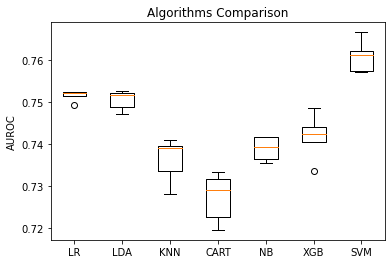
\includegraphics[width=7.5cm]{fig/chapter5/Algorithm Comparison (no SMOTE, SKFold).png}
  \caption{\footnotesize{Ten-fold cross-validation without \acrshort{SMOTE}}}
  \label{fig:skfoldnosmote}
\end{subfigure} \\
\begin{subfigure}{0.5\textwidth}
  \centering
  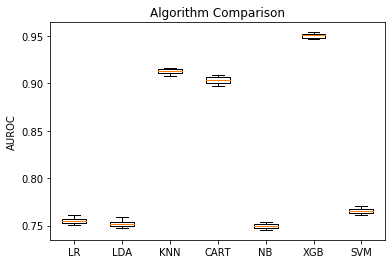
\includegraphics[width=7.5cm]{fig/chapter5/Algorithm Comparison (SMOTE, RSKFold).png}
  \caption{\footnotesize{Repeated 5-fold cross-validation with \acrshort{SMOTE}}}
  \label{fig:rskfoldsmote}
\end{subfigure} 
\begin{subfigure}{0.5\textwidth}
  \centering
  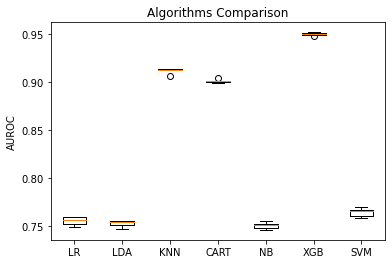
\includegraphics[width=7.5cm]{fig/chapter5/Algorithm Comparison (SMOTE, SKFold).png}
  \caption{\footnotesize{Ten-fold cross-validation with \acrshort{SMOTE}}}
  \label{fig:skfoldsmote}
\end{subfigure} \\
\end{tabular}
\caption{Comparison of the algorithms based on the \acrshort{AUC} criterion with/without \acrshort{SMOTE}}
\label{fig:comparison}
\end{figure}

{\hskip 1em} Figure \ref{fig:comparison} can also be analyzed from another point of view. Due to its synthetic behavior, utilizing \acrshort{SMOTE} balances the dataset in such a way that the \textit{Standard Deviation} of each algorithm is by far less than when no \acrshort{SMOTE} is used.

{\hskip 1em} Aside from confusion matrix, accuracy, and the \acrshort{AUC}, there is another classification evaluation method called \textbf{Cohen's Kappa}, a statistic to test interrater reliability, i.e., the extent of agreement among data collectors \cite{mchugh_interrater_2012}. Table \ref{tab:cohenskappa} demonstrates the value of Cohen's Kappa for each method. It can be seen that considering this criterion, \acrshort{XGB} achieves the highest Cohen's Kappa, which makes it the best algorithm among the rest.

\begin{table}[H]
\centering
\setlength\tabcolsep{50pt}
\caption{\label{tab:cohenskappa}Calculated Cohen's Kappa for the implemented models}
\begin{tabular}{@{}lc@{}}
\toprule
\thead{Algorithm}     & \thead{Cohen's Kappa}        \\ \midrule \midrule
\acrfull{CART}        & 0.683919                     \\ \midrule
\acrfull{XGB}         & 0.803587                     \\ \midrule
\acrfull{SVM}         & 0.380761                     \\ \midrule
\acrfull{LR}          & 0.359726                     \\ \midrule
\acrfull{NB}          & 0.308094                     \\ \midrule
\acrfull{LDA}         & 0.352173                     \\ \midrule
\acrfull{KNN}         & 0.672806                     \\
\bottomrule
\end{tabular}
\end{table}

\subsection{Computational Complexity}
There is another aspect of studying \acrlong{ML} algorithms and evaluating them: Computational Complexity, which gives an asymptotic upper bound to a function and is referred to as big-O notation. It bounds the growth of the running time from above and describes the code complexity using algebraic terms \cite{kearns_introduction_1994}. Table \ref{tab:bigonotation} shows the formulated computational complexity for the algorithms used in our work. \

{\hskip 1em} In calculating the big-O notation, only dominant terms, and not coefficients, matters. Regarding that, the common term in all the formulas of table \ref{tab:bigonotation} is $n$, which is the input size ($n=59190$). $d$ denotes the number of dimensions or features ($d=11$). In \acrshort{KNN}, parameter $k$ is the number of nearest neighbors taken into account ($k=25$), while in \acrshort{XGB}, it means the number of trees ($k=100$). Eventually, ${\lVert\mathrm{x}\rVert}_0$ stands for the number of non-missing entries in the training data (${\lVert\mathrm{x}\rVert}_0=59190$).

{\hskip 1em} Table \ref{tab:complexitytime} represents the running time of a single instance of the training set of each implemented algorithm. It can be recognized that \acrshort{SVM} has the longest running time that is understandable since it uses an internal five-fold cross-validation, which increases the running time exponentially. From the big-O notation point of view, it can also be concluded since the \acrshort{SVM} behavior corresponds to $n^2$, and $n$ is quite huge. Comparing an algorithm's big-O notation formula with its respective instance running time, considering the parameter values, proves that the calculated running times are as rational as expected.

\begin{table}[H]
\centering
\setlength\tabcolsep{50pt}
\caption{\label{tab:bigonotation}Training computational complexity of the algorithms}
\begin{tabular}{@{}lc@{}}
\toprule
\thead{Algorithm}     & \thead{Big-O Notation}        \\ \midrule \midrule
\acrfull{CART}        & $O(nlog(n)\times d)$          \\ \midrule
\acrfull{XGB}         & $O(kd{\lVert\mathrm{x}\rVert}_0log(n))$   \\ \midrule
\acrfull{SVM}         & $O(n^2)$                      \\ \midrule
\acrfull{LR}          & $O(nd)$                       \\ \midrule
\acrfull{NB}          & $O(nd)$                       \\ \midrule
\acrfull{LDA}         & $O(nd^2)$                     \\ \midrule
\acrfull{KNN}         & $O(nd+kn)$                    \\
\bottomrule
\end{tabular}
\end{table}

\begin{table}[H]
\centering
\setlength\tabcolsep{30pt}
\caption{\label{tab:complexitytime}The running time of a single training set instance}
\begin{tabular}{@{}lc@{}}
\toprule
\thead{Algorithm}     & \thead{Instance (ms)}         \\ \midrule \midrule
\acrfull{CART}        & 0.00405                       \\ \midrule
\acrfull{XGB}         & 0.42355                       \\ \midrule
\acrfull{SVM}         & 16.7944                       \\ \midrule
\acrfull{LR}          & 0.02082                       \\ \midrule
\acrfull{NB}          & 0.00162                       \\ \midrule
\acrfull{LDA}         & 0.00282                       \\ \midrule
\acrfull{KNN}         & 0.00615                       \\
\bottomrule
\end{tabular}
\end{table}